\documentclass{article}
\usepackage[ruled,vlined]{algorithm2e}
\usepackage[bottom=8em]{geometry}
\usepackage{amsmath, amssymb, amsthm, enumerate, hyperref}
\usepackage{color}
\usepackage{setspace}
\usepackage{fancyhdr,lastpage}
\usepackage{url}
\usepackage{tabularx}
\usepackage{tikz}
\pagestyle{fancy}
\lhead{\footnotesize Problem Set 1}
\chead{}
\rhead{\footnotesize CS 4150 - Fall 2020}
\lfoot{}
\cfoot{\small \thepage/\pageref*{LastPage}}
\rfoot{}

\usepackage{graphicx}

\newcommand{\pname}[1]{\textnormal{\textsc{#1}}}

\newtheorem*{theorem}{Theorem}
\newtheorem{definition}{Definition}
\newtheorem*{lemma}{Lemma}


\begin{document}

{\it Please enter your name and uID below.}

\vspace{3em}

\makebox[4.3cm]{Name: Qianlang Chen}
\par
\makebox[4.3cm]{uID: u1172983}
\par

\vfill

\subsubsection*{Submission notes}
\begin{itemize}
  \item Due at 11:59 pm on Friday, September 11.
  \item Solutions must be typeset using one of the template files. For each problem, your answer must fit in the space provided (e.g. not spill onto the next page) *without* space-saving tricks like font/margin/line spacing changes.
  \item Upload a PDF version of your completed problem set to Gradescope.
  \item Teaching staff reserve the right to request original source/tex files during the grading process, so please retain these until an assignment has been returned.
  \item Please remember that for problem sets, collaboration with other students must be limited to a high-level discussion of solution strategies. If you do collaborate with other students in this way, you must identify the students and describe the nature of the collaboration. You are not allowed to create a group solution, and all work that you hand in must be written in your own words. Do not base your solution on any other written solution, regardless of the source.
\end{itemize}

\pagebreak


\begin{enumerate}

  \item (Big-$\Theta$) Proof: to use the definition of Big-$\Theta$, we need to show both $\log(n!) = O[n\log(n)]$ and $\log(n!) = \Omega[n\log(n)]$.

    \begin{itemize}
      \item \textbf{Part I:} show that $\log(n!) = O[n\log(n)]$, that is, there exist constants $c, k > 0$ such that $\log(n!) \le c \cdot n\log(n)$ for all $n \ge k$.

        Proof: let $c = 1$ and $k = 100$. Now, for all $n \ge 100$, we have
        \begin{displaymath}
          \begin{aligned}
            \log(n!)      & \le 1 \cdot n\log(n)                                        \\
            \log(n!)      & \le \log(n^n)                                               \\
            10^{\log(n!)} & \le 10^{\log(n^n)}                                          \\
            n!            & \le n^n                                                     \\
            \underbrace{n \cdot (n-1) \cdot (n-2) \cdots 1}_{n\text{ items}}
                          & \le \underbrace{n \cdot n \cdot n\cdots n}_{n\text{ items}}
          \end{aligned}
        \end{displaymath}
        (Since each factor gets smaller on the left-hand side whereas it stays constant on the right-hand side.)

        Therefore, by definition of Big-Oh, $\log(n!) = O[n\log(n)]$.

      \item \textbf{Part II:} show that $\log(n!) = \Omega[n\log(n)]$, that is, there exist constants $c, k > 0$ such that $\log(n!) \ge c \cdot n\log(n)$ for all $n \ge k$.

        Proof: let $c = \frac{1}{4}$ and $k = 100$. Now, for all $n \ge 100$, we have
        \begin{displaymath}
          \begin{aligned}
            \log(n!)      & \ge \frac{1}{4} \cdot n\log(n)                                                      \\
            \log(n!)      & \ge \log(n^{\frac{n}{4}})                                                           \\
            10^{\log(n!)} & \ge 10^{\log(n^{n/4})}                                                              \\
            n!            & \ge n^\frac{n}{4}                                                                   \\
            n!            & \ge (\sqrt{n})^{\frac{n}{2}}                                                        \\
            \underbrace{n \cdot (n-1) \cdots (\frac{n}{2}+1)}_{\frac{n}{2}\text{ items}}
            \cdot \frac{n}{2} \cdots 1
                          & \ge \underbrace{\sqrt{n} \cdot \sqrt{n} \cdots \sqrt{n}}_{\frac{n}{2}\text{ items}}
          \end{aligned}
        \end{displaymath}
        (Since $\frac{n}{2} > \sqrt{n}$ for all $n \ge 100$, meaning that the first $\frac{n}{2}$ factors on the left-hand side are all greater than $\sqrt{n}$.)

        Therefore, by definition of Big-$\Omega$, $\log(n!) = \Omega[n\log(n)]$.
    \end{itemize}

    Since we have managed to show both $\log(n!) = O[n\log(n)]$ and $\log(n!) = \Omega[n\log(n)]$, by definition of Big-$\Theta$, $\log(n!) = \Theta[n\log(n)]$. $\square$

    \pagebreak

  \item (Party Planning)

    % answer question 2 here

    \pagebreak

  \item (Amortized ArrayList) Proof: the {\tt ArrayList} needs to resize once the number of contained elements reaches $n$; so does it once it reaches $(n + c), (n + 2c)$, and so on. During $k$ {\tt add\_end()} calls, the {\tt ArrayList} has to resize approximately $\frac{k-n}{c}$ times, since each resize gives it the space for $c$ additional elements. (The error in the number of times it needs to resize due to $(k - n)$ not being a multiple of $c$ will get smaller as $k$ gets large.) Since the {\tt ArrayList} needs to resize so many times when $k$ is large, the run time of $k$ {\tt add\_end()} function calls is dominated by the time spent resizing and copying the elements:
    $$T(k) \approx \underbrace{n + (n + c) + (n + 2c) + \cdots}_{\sim (k-n) / c\text{ items}}$$

    We can evaluate/approximate the above sum by visualizing it with the following triangle:
    $$
      \sim \frac{k-n}{c}\text{ items} \begin{cases}
         & n                                                               \\
         & n + c                                                           \\
         & n + c + c                                                       \\
         & \vdots                                                          \\
         & \underbrace{n + c + c + \cdots + c}_{\sim (k-n)/c\text{ items}}
      \end{cases}
      \begin{aligned}
        \implies T(k) & \approx \text{The area of the triangle}                                             \\
                      & \approx (\frac{k-n}{c}) \cdot n + \frac{1}{2}(\frac{k-n}{c})(\frac{k-n}{c}) \cdot c \\
                      & \approx \boxed{\frac{kn-n}{c} + \frac{k^2 - 2kn + n^2}{2c}}
      \end{aligned}
    $$

    Since $T(k) \ge \frac{1}{2c} \cdot k^2$ for all $k \ge 2n$, by definition of Big-$\Omega$, $T(k) = \Omega(k^2)$. Therefore, $T(k)$ is not $O(k)$. $\square$

    \pagebreak

  \item (Sorting) Proof: the first thing to observe is that the run time of the {\tt sorted()} function is $O(r)$ in the worst case, where $r$ is the value of the {\tt right} input.

    Now, let us consider the worse-case scenario for the entire algorithm.

      {\tt mergesort2()} is mostly the same as a regular merge-sort, and the only difference is that this new algorithm calls the {\tt sorted()} function at each recursion level before the regular routine. In the worse-case, the {\tt sorted()} function returns {\tt false} every time, forcing the algorithm to do the regular merge-sort. Following this idea, let $T(n, l, r)$ represent the run time of {\tt mergesort2()} with data size $n$ and values of the arguments {\tt left} and {\tt right} being $l$ and $r$, and we have
    $$
      \begin{aligned}
        T(n, l, r) & = T_{\text{sorted}}(r) + T(\frac{n}{2}, l, \frac{l+r}{2})
        + T(\frac{n}{2}, \frac{l+r}{2}, r) + T_{\text{merge}}(n)                                          \\
                   & = O(r) + T(\frac{n}{2}, l, \frac{l+r}{2}) + T(\frac{n}{2}, \frac{l+r}{2}, r) + O(n); \\
        T(n)       & = T(n, 0, n)
      \end{aligned}
    $$
    This is better visualized with the following recursion tree, where the values in each node is formatted as $\boxed{T_{\text{sorted}}(r) + T_{\text{merge}}(n)}$:

    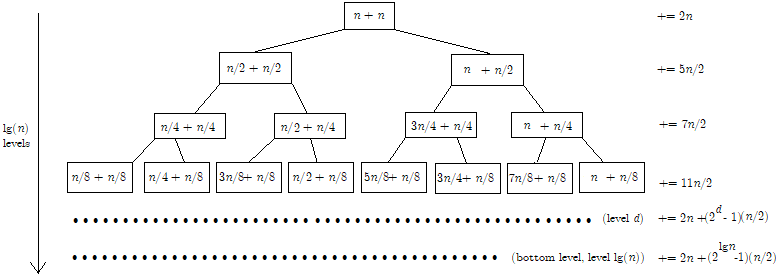
\includegraphics[width=\linewidth]{./images/q4_1.png}

    The total run time of {\tt mergesort2()} is the sum of the run times for all levels, the values to the right of the tree:
    $$
      \begin{aligned}
        T(n) & = \overbrace{2n + \frac{5n}{2} + \frac{7n}{2} + \frac{11n}{2} + \cdots}^{\log_2(n)\text{ items}}      \\
             & = 2n + (2n + \frac{n}{2}) + (2n + \frac{3n}{2}) + (2n + \frac{7n}{2})
        + \cdots + (2n + (2^{\log_2(n)}-1)\frac{n}{2})                                                               \\
             & = \log_2(n) \cdot 2n + (\frac{n}{2} + \frac{3n}{2} + \frac{7n}{2}
        + \cdots + (n - 1)\frac{n}{2})                                                                               \\
             & = 2n\log_2(n) + (\frac{2n}{2} - \frac{n}{2} + \frac{4n}{2} - \frac{n}{2} + \frac{8n}{2} - \frac{n}{2}
        + \cdots+ n\frac{n}{2} - \frac{n}{2})                                                                        \\
             & = 2n\log_2(n) + \frac{n}{2} \cdot (2 + 4 + 8 + \cdots + n) - \frac{n}{2} \cdot \log_2(n)              \\
             & = \frac{3n\log_2(n)}{2} + n(n - 1) = \boxed{\frac{3n\log_2(n)}{2} + n^2 - n}
      \end{aligned}
    $$

    Now, since we have $T(n) \le 2n^2$ for all $n \ge 1$, by definition of Big-Oh, $T(n) = O(n^2)$. $\square$

    \pagebreak

  \item (Erickson 1.37)

    % answer question 5 here

\end{enumerate}

\end{document}
